%%%%%%%%%%%%%%%%%%%%%%%%%%%%%%%%%%%%%%%%%
% Beamer Presentation
% LaTeX Template
% Version 1.0 (10/11/12)
%
% This template has been downloaded from:
% http://www.LaTeXTemplates.com
%
% License:
% CC BY-NC-SA 3.0 (http://creativecommons.org/licenses/by-nc-sa/3.0/)
%
%%%%%%%%%%%%%%%%%%%%%%%%%%%%%%%%%%%%%%%%%

%----------------------------------------------------------------------------------------
%	PACKAGES AND THEMES
%----------------------------------------------------------------------------------------

\documentclass{beamer}

\mode<presentation> {

% The Beamer class comes with a number of default slide themes
% which change the colors and layouts of slides. Below this is a list
% of all the themes, uncomment each in turn to see what they look like.

%\usetheme{default}
%\usetheme{AnnArbor}
%\usetheme{Antibes}
%\usetheme{Bergen}
%\usetheme{Berkeley}
%\usetheme{Berlin}
%\usetheme{Boadilla}
%\usetheme{CambridgeUS}
%\usetheme{Copenhagen}
%\usetheme{Darmstadt}
%\usetheme{Dresden}
%\usetheme{Frankfurt}
%\usetheme{Goettingen}
%\usetheme{Hannover}
%\usetheme{Ilmenau}
\usetheme{JuanLesPins}
%\usetheme{Luebeck}
%\usetheme{Madrid}
%\usetheme{Malmoe}
%\usetheme{Marburg}
%\usetheme{Montpellier}
%\usetheme{PaloAlto}
%\usetheme{Pittsburgh}
%\usetheme{Rochester}
%\usetheme{Singapore}
%\usetheme{Szeged}
%\usetheme{Warsaw}

% As well as themes, the Beamer class has a number of color themes
% for any slide theme. Uncomment each of these in turn to see how it
% changes the colors of your current slide theme.

%\usecolortheme{albatross}
%\usecolortheme{beaver}
%\usecolortheme{beetle}
%\usecolortheme{crane}
%\usecolortheme{dolphin}
%\usecolortheme{dove}
%\usecolortheme{fly}
%\usecolortheme{lily}
%\usecolortheme{orchid}+
%\usecolortheme{rose}
%\usecolortheme{seagull}
%\usecolortheme{seahorse}
%\usecolortheme{whale}
%\usecolortheme{wolverine}

%\setbeamertemplate{footline} % To remove the footer line in all slides uncomment this line
\setbeamertemplate{footline}[page number] % To replace the footer line in all slides with a simple slide count uncomment this line

\setbeamertemplate{navigation symbols}{} % To remove the navigation symbols from the bottom of all slides uncomment this line
}

\usepackage{graphicx} % Allows including images
\usepackage{booktabs} % Allows the use of \toprule, \midrule and \bottomrule in tables

\usepackage[ngerman]{babel}
\usepackage[utf8]{inputenc}

%----------------------------------------------------------------------------------------
%	TITLE PAGE
%----------------------------------------------------------------------------------------

\title[Erkennung von erkrankten Nutzpflanzen]{Erkennung von erkrankten Nutzpflanzen anhand von Sentinel-2-Multispektralaufnahmen} % The short title appears at the bottom of every slide, the full title is only on the title page

\author{Simon Hüning} % Your name

\institute[] % Your institution as it will appear on the bottom of every slide, may be shorthand to save space
{
Universität Leipzig \\ % Your institution for the title page
\medskip
}
\date{\today} % Date, can be changed to a custom date

\begin{document}

\begin{frame}
\titlepage % Print the title page as the first slide
\end{frame}

\begin{frame}
\frametitle{Inhalt} % Table of contents slide, comment this block out to remove it
\tableofcontents % Throughout your presentation, if you choose to use \section{} and \subsection{} commands, these will automatically be printed on this slide as an overview of your presentation
\end{frame}

%----------------------------------------------------------------------------------------
%	PRESENTATION SLIDES
%----------------------------------------------------------------------------------------

\begin{frame}\section{Motivation}\frametitle{Motivation}
\begin{minipage}{0.5\textwidth}
	\begin{itemize}
		\item Frühzeitige Erkennung von Infizierungen sind eine große Herausforderung der Agrarindustrie
		\item Späte Identifikation von infizierten Nutzpflanzen sorgt für Ertragsverluste
		\item Meist zeigen sich sichtbare Symptome erst im fortgeschrittenen Stadium
	\end{itemize}
\end{minipage}
\hspace{1em}
\begin{minipage}{0.4\textwidth}
	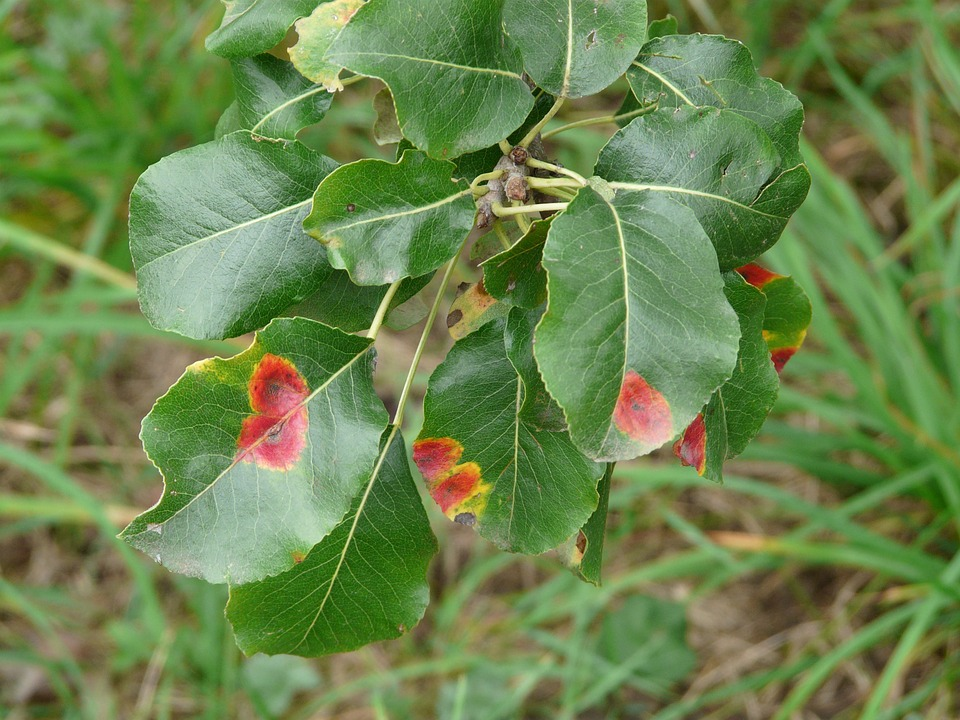
\includegraphics[width=1\linewidth]{pics/befall.png}
\end{minipage}
\end{frame}

%------------------------------------------------

\begin{frame}\section{Zielsetzung}\frametitle{Zielsetzung}
	\begin{itemize}
		\item Chlorophyllgehalt ist ein Indikator für Gesundheits-/Stressstatus
		\item Durch spektrale Aufnahmen messbar
		\item Keine sichtbaren Symptome nötig
	\end{itemize}
	Zielsetzung: Überwachte Lernverfahren können darauf trainiert werden, mit hoher Genauigkeit (über 90\%) Krankheiten zu klassifizieren.
\end{frame}

%------------------------------------------------
\begin{frame}\section{Sentinel-2}\frametitle{Sentinel-2}
\begin{minipage}{0.5\textwidth}
	\centering
	\begin{itemize}
		\item Satelliten zur Erdüberwachung (Land, Meer, Atmospäre)
		\item Sentinel-2-Paar ausgestattet mit multispektralen Messinstrumenten
		\item Erzeugt alle 5 Tage neue Aufnahmen
	\end{itemize}
	\vspace{1em}
	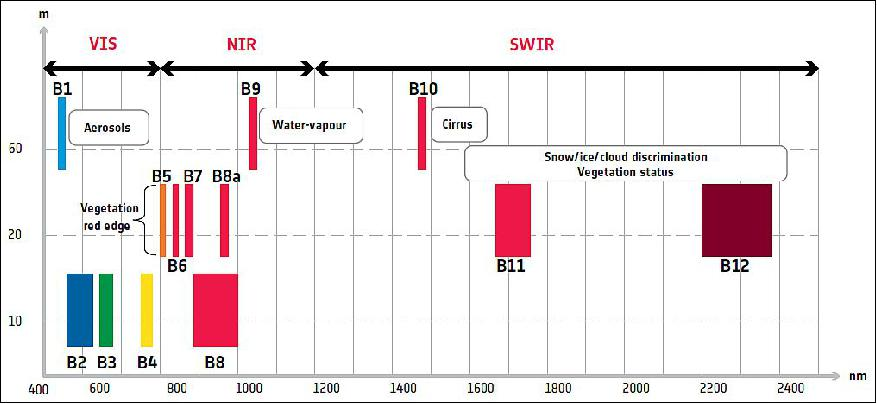
\includegraphics[width=0.9\linewidth]{pics/sentinel-2-bands.png}
\end{minipage}
\begin{minipage}{0.4\textwidth}
	\centering
	
\includegraphics[width=0.5\linewidth]{pics/copernicus-logo.png}\\
	\vspace{3em}
	\includegraphics[width=1\linewidth]{pics/Sentinel-2-scanning.png}
\end{minipage}
\end{frame}

%------------------------------------------------

\begin{frame}\frametitle{Copernicus Open Access Hub}
	\centering
	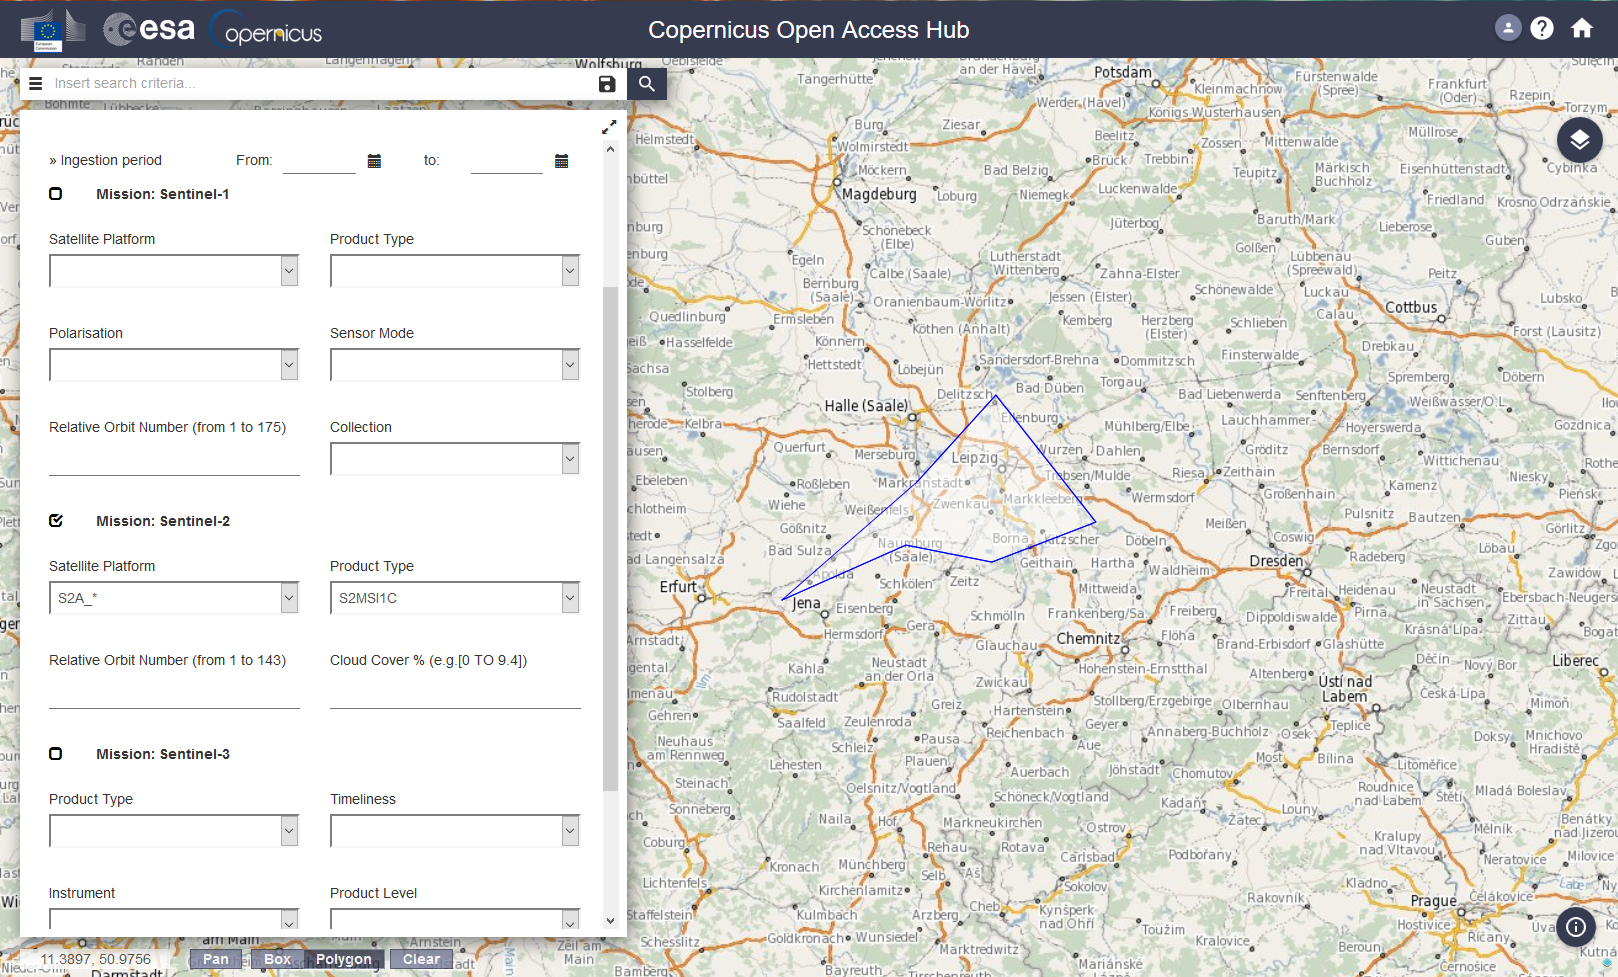
\includegraphics[width=0.7\textwidth,height=0.6\textheight]{pics/scihub-query.PNG}
	\hspace{.5em}
	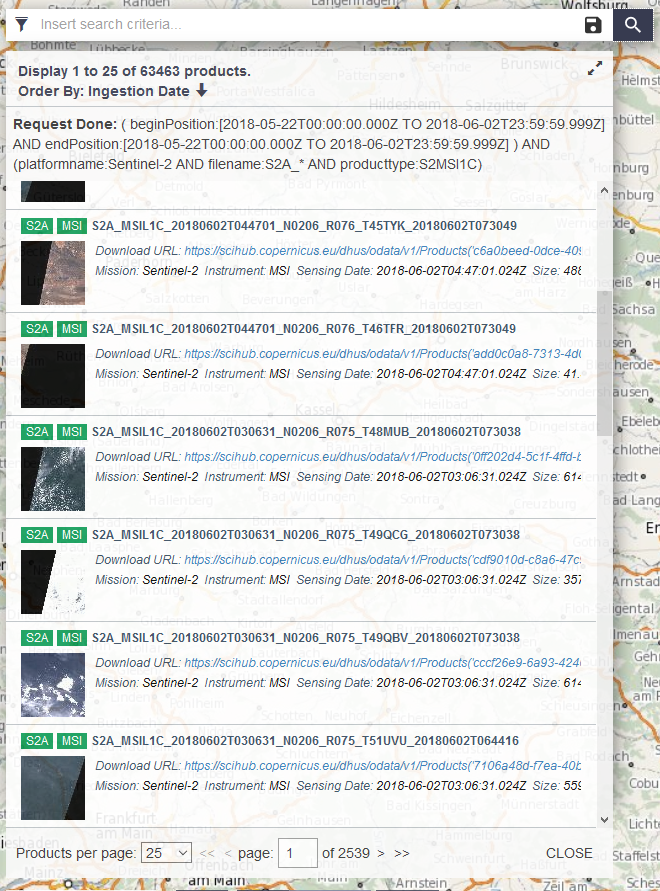
\includegraphics[width=0.25\textwidth,height=0.6\textheight]{pics/scihub-productlist.PNG}
\end{frame}

%------------------------------------------------

\begin{frame}\section{Multiclass SVM}\frametitle{Multiclass SVM}
	\begin{itemize}
		\item Erweiterung einer SVM, wenn mehr als 2 Klassen vorhanden sind
		\item Klassifizierung durch Support Vektoren
		\item Schnelle Klassifizierung, da die benötigten Parameter nur auf wenigen Support Vektoren basieren
		\item Hohe Generalisierungsfähigkeit und kann gut auf reale Probleme angesetzt werden
	\end{itemize}
\end{frame}

%------------------------------------------------

\begin{frame}\section{Convolutional Neural Network}\frametitle{Convolutional Neural Network}
	\begin{itemize}
		\item Durch Visuellen Cortex inspiriert
		\item Gute Ergebnisse bei Bilddaten
		\item Weniger Verbindungen zwischen Neuronen als vollständig verbundene KNNs (daher gut bei großen Eingabedatenmengen)
	\end{itemize}
	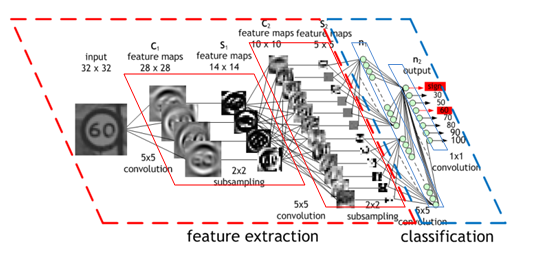
\includegraphics[width=1\textwidth]{pics/cnn.PNG}
\end{frame}


%------------------------------------------------

\begin{frame}\section{Probleme}\frametitle{Probleme}
	\begin{itemize}
		\item Datenlage
		\item Wetter
		\item Größe der Daten (Sentinelaufnahmen 10980x10980px groß)
		%\item Intervall bis die Satelliten die Erde abgemessen haben, könnte zu groß sein
	\end{itemize}
\end{frame}

%------------------------------------------------

\begin{frame}\section{Zeitplan}\frametitle{Zeitplan}
\begin{tabular}{l l}
1. April & Beginn \\
5. Juni & Themenvorstellung\\
Anfang Juni & Anmeldung\\
Ende Juni & Fertigstellung Prototyp\\
Mitte August & Zwischenvortrag\\
Mitte November & Abschlusspräsentation
\end{tabular}
\end{frame}

%------------------------------------------------

\begin{frame}\frametitle{Bildquellen}
\begin{itemize}
\item Sentinel-2-Abbildung\\
\url{https://www.esa.int/var/esa/storage/images/esa_multimedia/images/2008/04/sentinel-2/9940106-2-eng-GB/Sentinel-2\_node\_full\_image\_2.jpg}
\item Copernicus-Logo\\
\url{http://copernicus.eu/sites/all/themes/copernicus/logo.png}
\item Befall\\
\url{https://cdn.pixabay.com/photo/2012/10/06/02/20/birnbaum-leaves-59904\_960\_720.jpg}
\item Sentinel-2-Bänder\\
\url{https://directory.eoportal.org/documents/163813/3507495/Sentinel2\_Auto16.jpeg}
\item Convolutional Neural Network\\
\url{https://upload.wikimedia.org/wikipedia/commons/6/63/Typical\_cnn.png}
\end{itemize}
\end{frame}

%------------------------------------------------

\begin{frame}
\centerline{Vielen Dank für Ihre Aufmerksamkeit.}
\Huge{\centerline{Fragen?}}
\end{frame}

%----------------------------------------------------------------------------------------

\end{document} 